\documentclass[a4paper,11pt]{article}
\usepackage{amsmath,amssymb}
\usepackage[a4paper,left=19mm,right=19mm,top=40mm,bottom=40mm]{geometry}
\usepackage{txfonts}
\usepackage{kotex}
\usepackage{graphicx}
\usepackage{algorithm}
\usepackage{algpseudocode}
\usepackage{fancyvrb}

\begin{document}
\title{자료구조 HW10-지하철}
\author{B935394 컴퓨터공학과 장준희}
\maketitle
\newpage
\section{최단거리 알고리즘-Dijkstra}
\subsection{선택한 이유}
\ \ 우선은 교재의 알고리즘이 다익스트라 알고리즘이라 선택한 것이 컸다. 한 점에서 시작해서 모든 점까지의 최단시간을 구하는데, 두 점 사이의 공평한 점을 찾는데 있어서는 모든 점까지의 최단시간을 구하는게 필요하다고 생각했다. BellmanFord 알고리즘도 교재에 있었지만, 거리가 음수인 경우는 없었기 때문에 굳이 선택하지 않았다. 
\subsection{알고리즘의 이해}
\ \ 사실 알고리즘이 처음에 이해가 잘 안가서 처음에는 책에 나와있는 예시를 가지고 천천히 따라가봤었다. 그러고도 조금은 아리까리해서 아예 예시를 하나 만들어서 한줄한줄 따라가보았다.
\begin{figure}[h]
\begin{center}
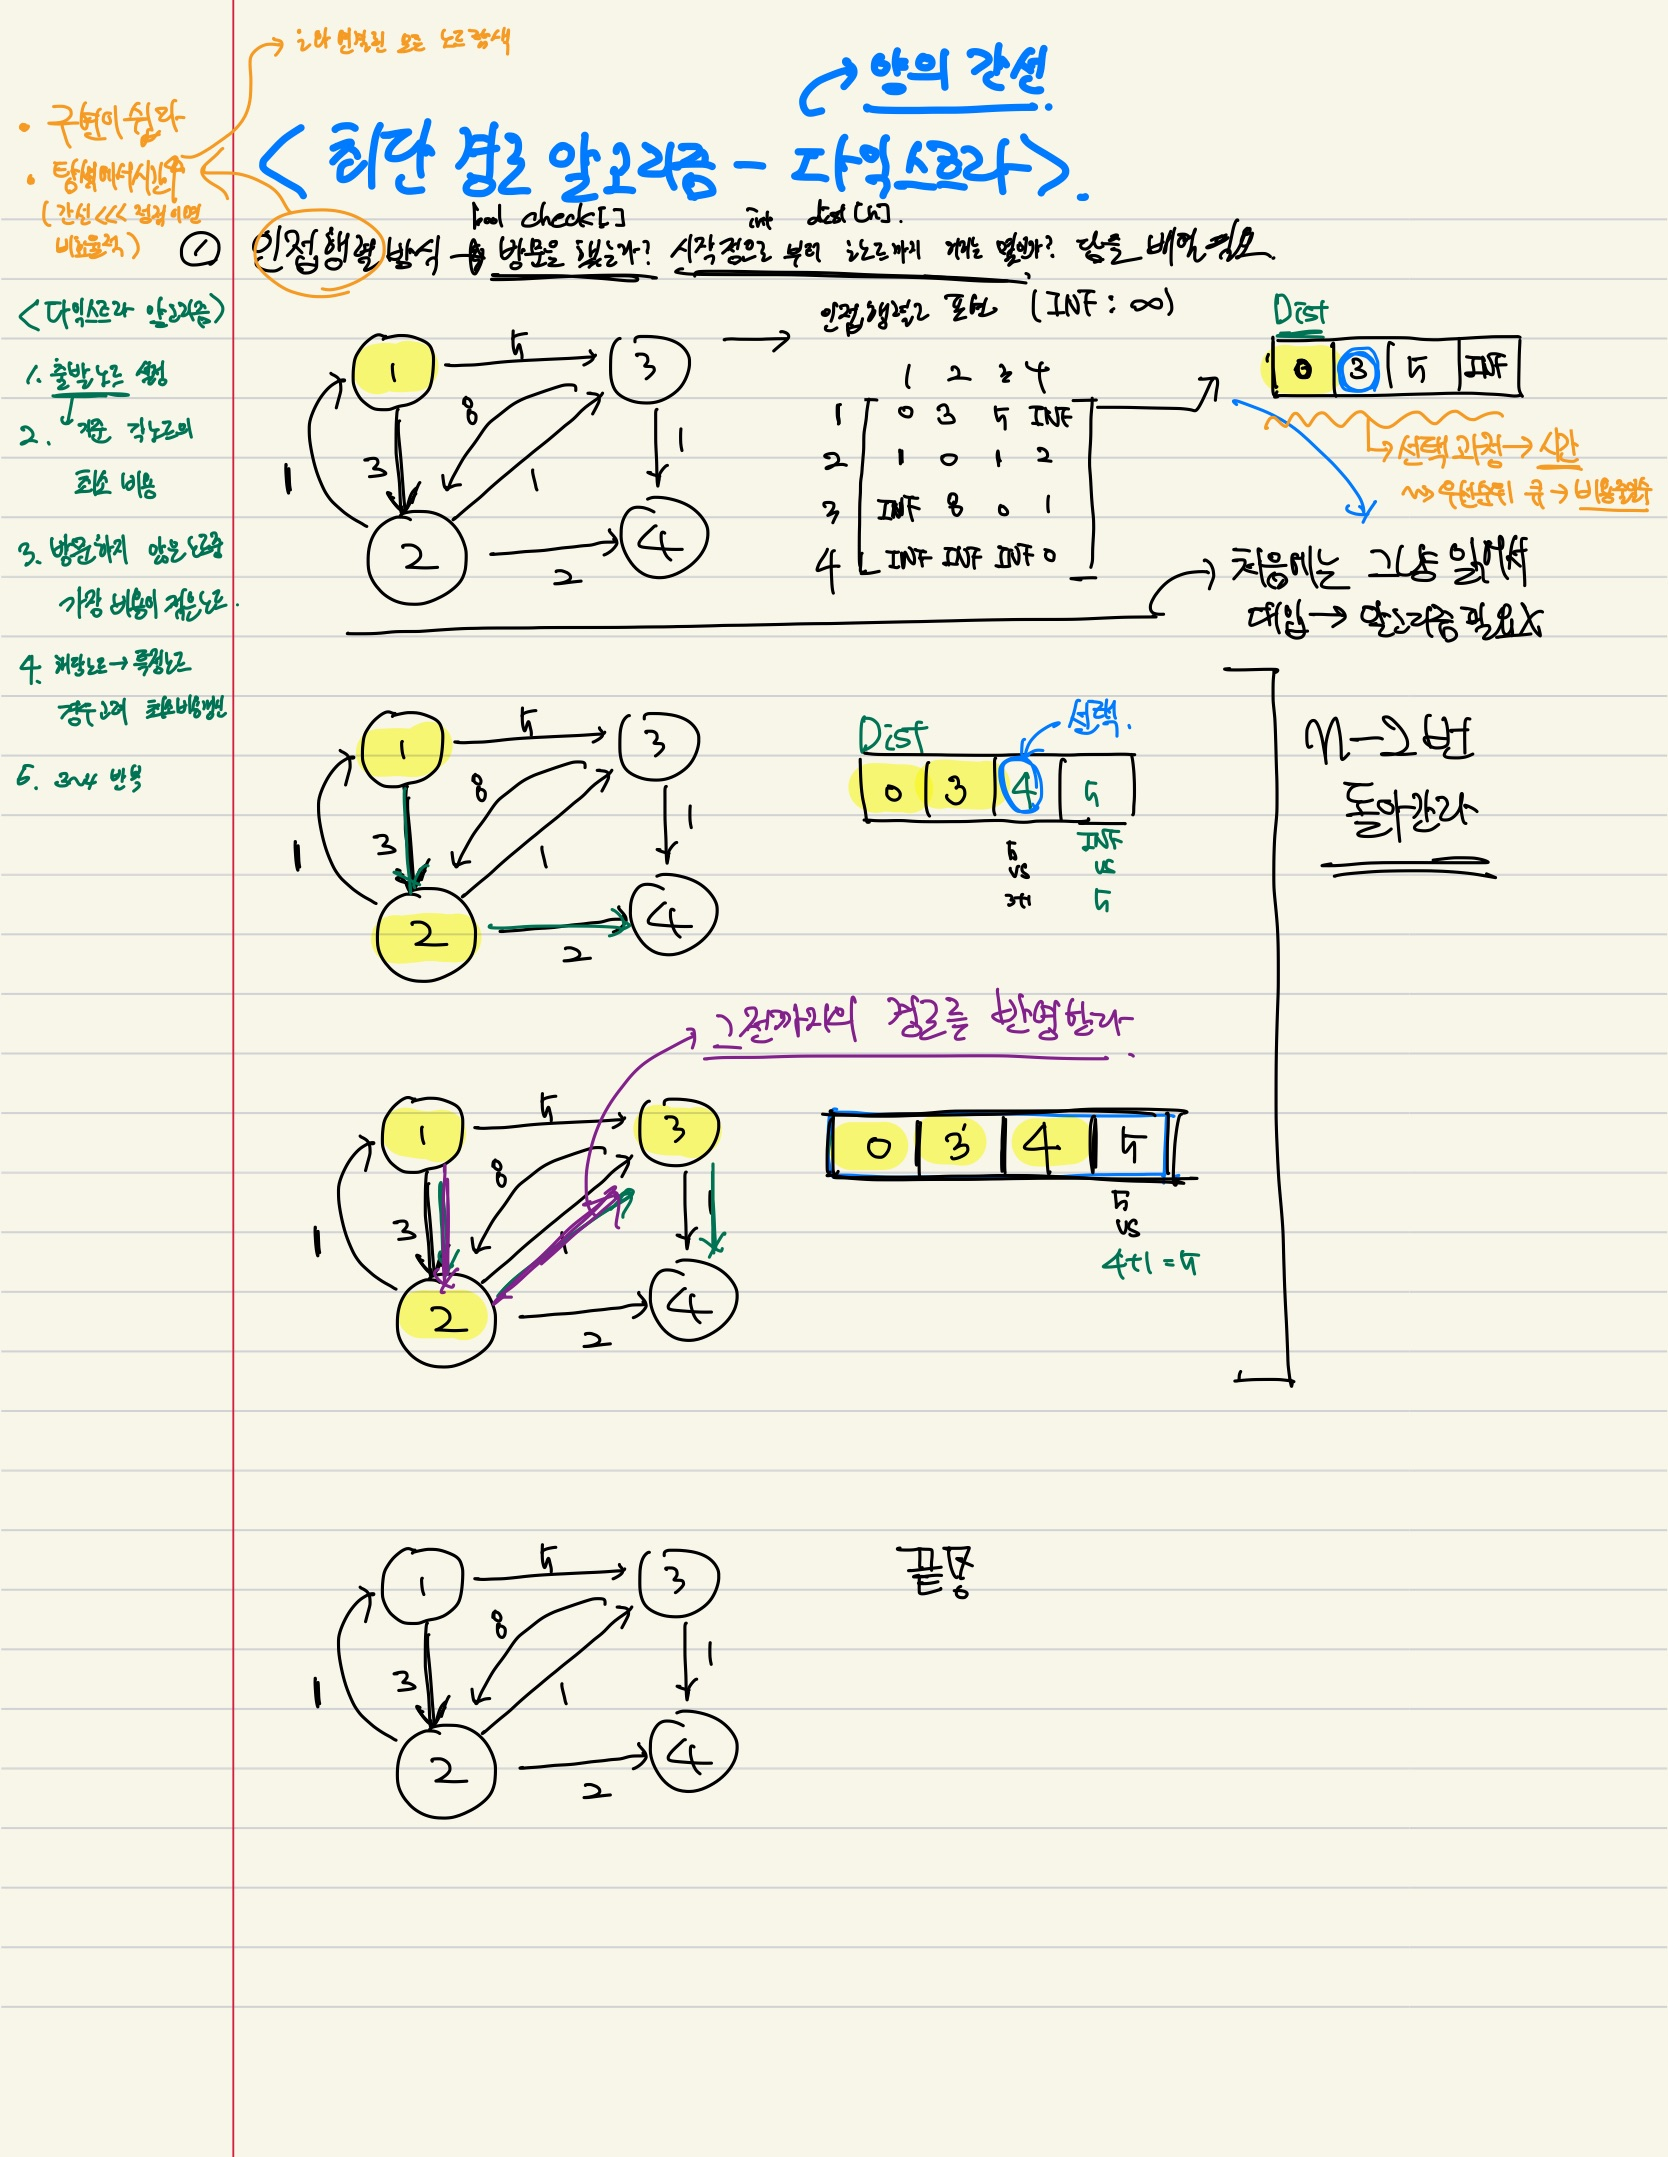
\includegraphics[width=0.6\textwidth]{DijstraMatrix}
\caption{Dijkstra-Matrix}
\label{fig:fig1}
\end{center}
\end{figure}


해보고나니, 한 점(Q)에 대해서 현재까지 알려진 거리(d1)와, 최단거리가 구해진 점(P)까지의 거리와 그 점(P)으로부터 한 점(Q)까지의 거리의 합(d2)을 비교하여 둘(d1,d2) 중 더 작은 값을 저장하는 것이였다. 알고리즘에 대해 이해하기 위해 구글링을 하다보니, 인접리스트를 통해 구현된 그래프와 큐를 이용한다면 더 빠르게 구할 수 있다는 사실을 알게되었다. 문제는 역시나 또 코드든 설명이든 읽기만 해서는 이해가 안간다는 것이였다. 그래서 다시 한 번 예시를 들어서 한줄한줄 따라가기 시작했다. 
\begin{figure}[h]
\begin{center}
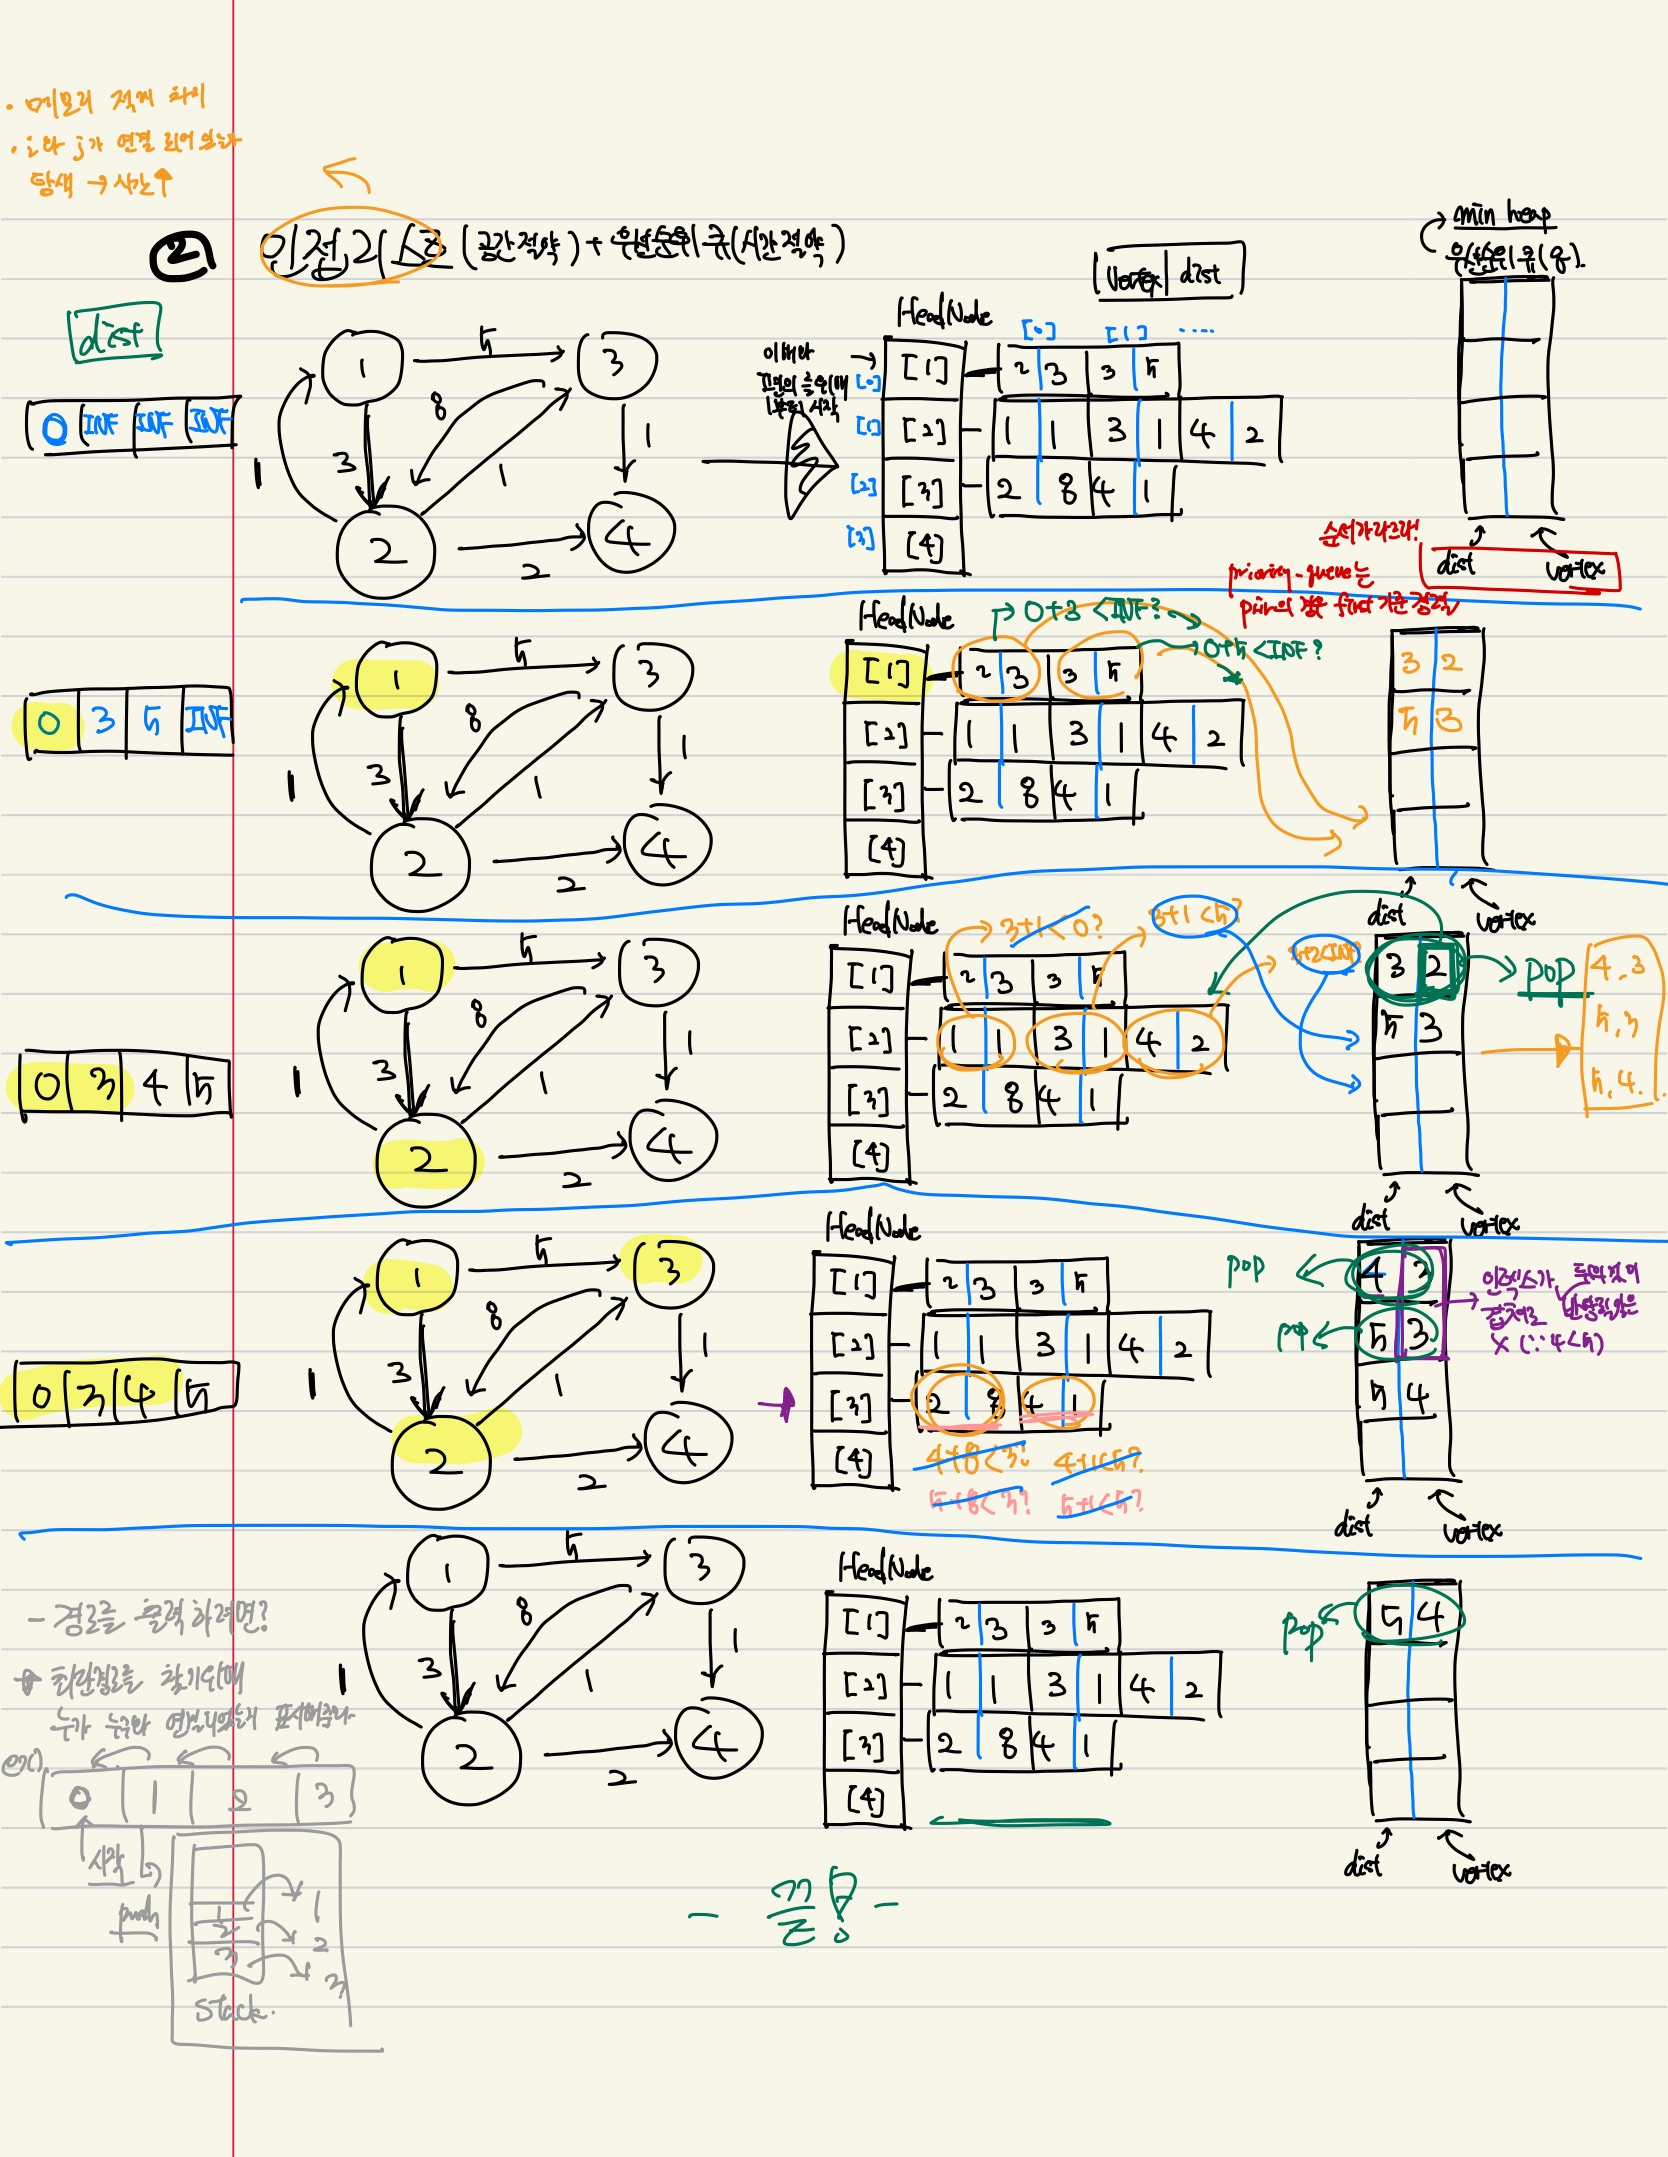
\includegraphics[width=0.6\textwidth]{DijstraList}
\caption{Dijkstra-List}
\label{fig:fig2}
\end{center}
\end{figure}


하기 전에 들었던 생각은, 인접행렬에서와 같이 check하는 배열이 따로 있는 것도 아닌데 겹치면 어떡하나 하는 의문이였다. 들어본 예시의 4번째 상황을 하면서 해소가 되었는데, 어차피 같은 인덱스에 대해 다른 거리들이 있더라도 반영되는 것은 그 중 제일 작은 값만 반영된다는 것이였다. 
\newpage
\section{클래스의 설계,\ 그래프 구성 방식}
\ \ 알고리즘을 정하기도 전에 음에 했던 설계는 다음과 같았다.
\begin{figure}[h]
\begin{center}
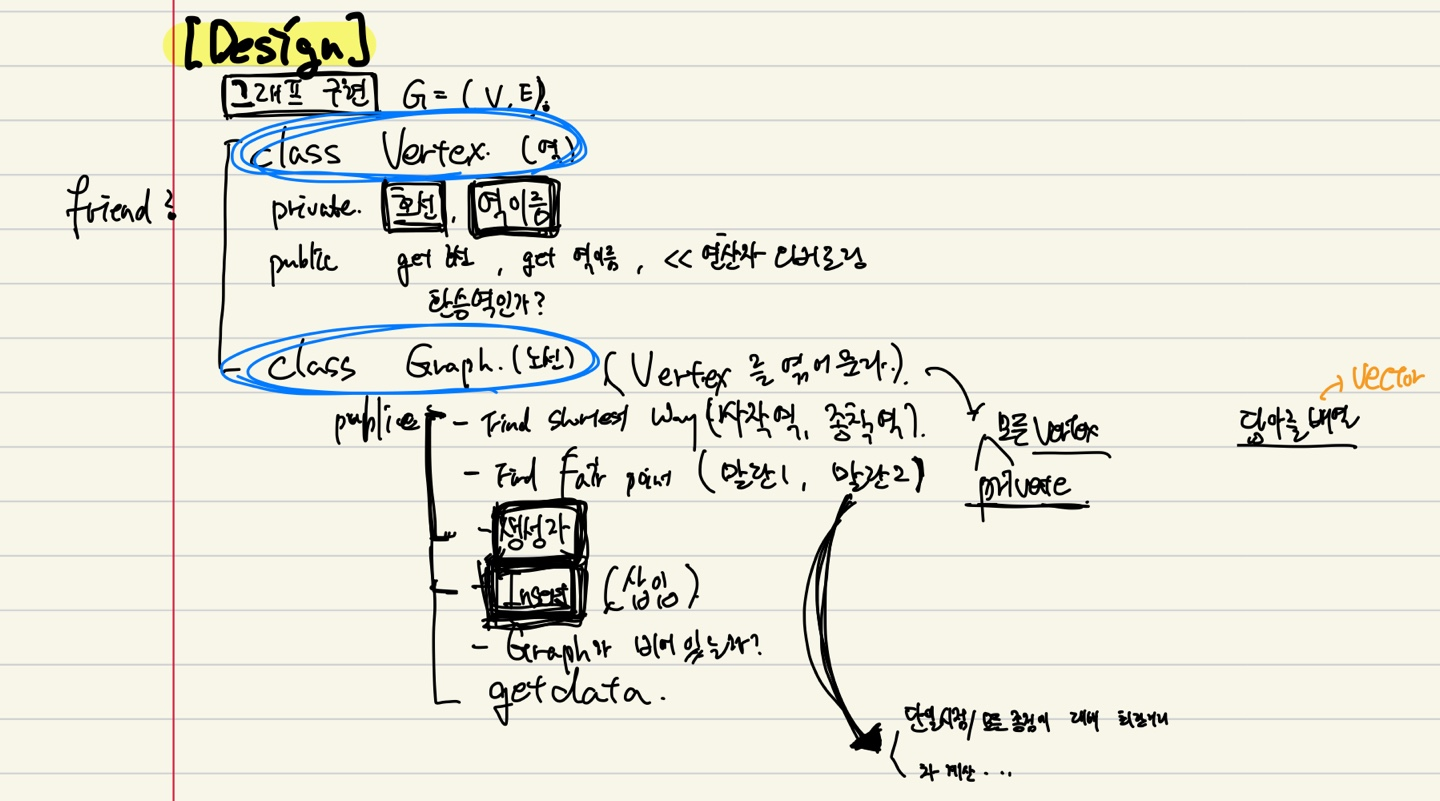
\includegraphics[width=0.6\textwidth]{design}
\caption{Design}
\label{fig:fig3}
\end{center}
\end{figure}


그래프는 인접리스트로 표현할 생각이였고, 그래서 간선은 없이 정점만 다룰 수 있으면 되었다. 우선 정점에는 private 영역에 호선, 역이름을 넣어두고 public에는 그걸 꺼내서 볼 수 있게 해주는 함수, 그리고 출력을 위해서 $<<$연산자 오버로딩 정도면 충분하다고 생각했다. 

그래프에는, private영역에는 인접리스트, 모든 정점을 담아둘 배열 정도면 충분하고 public영역에 생성자, 삽입함수, 그래프가 있는지 없는지 여부, 최단거리 구하는 함수, 두 점으로 부터 공평한 점을 찾는 함수 정도면 충분하다고 생각했다.(getData함수는 무슨 함수인지 모르겠다. 아마도 그래프를 보여주려고 했던 것 같다.) 

그래프를 인접리스트로 어떻게 표현할까를 고민하기 시작했었다. 그래서 처음에는 또 예시를 들어서 간단하게 표현해봤었다.

\begin{figure}[!h]
\begin{center}
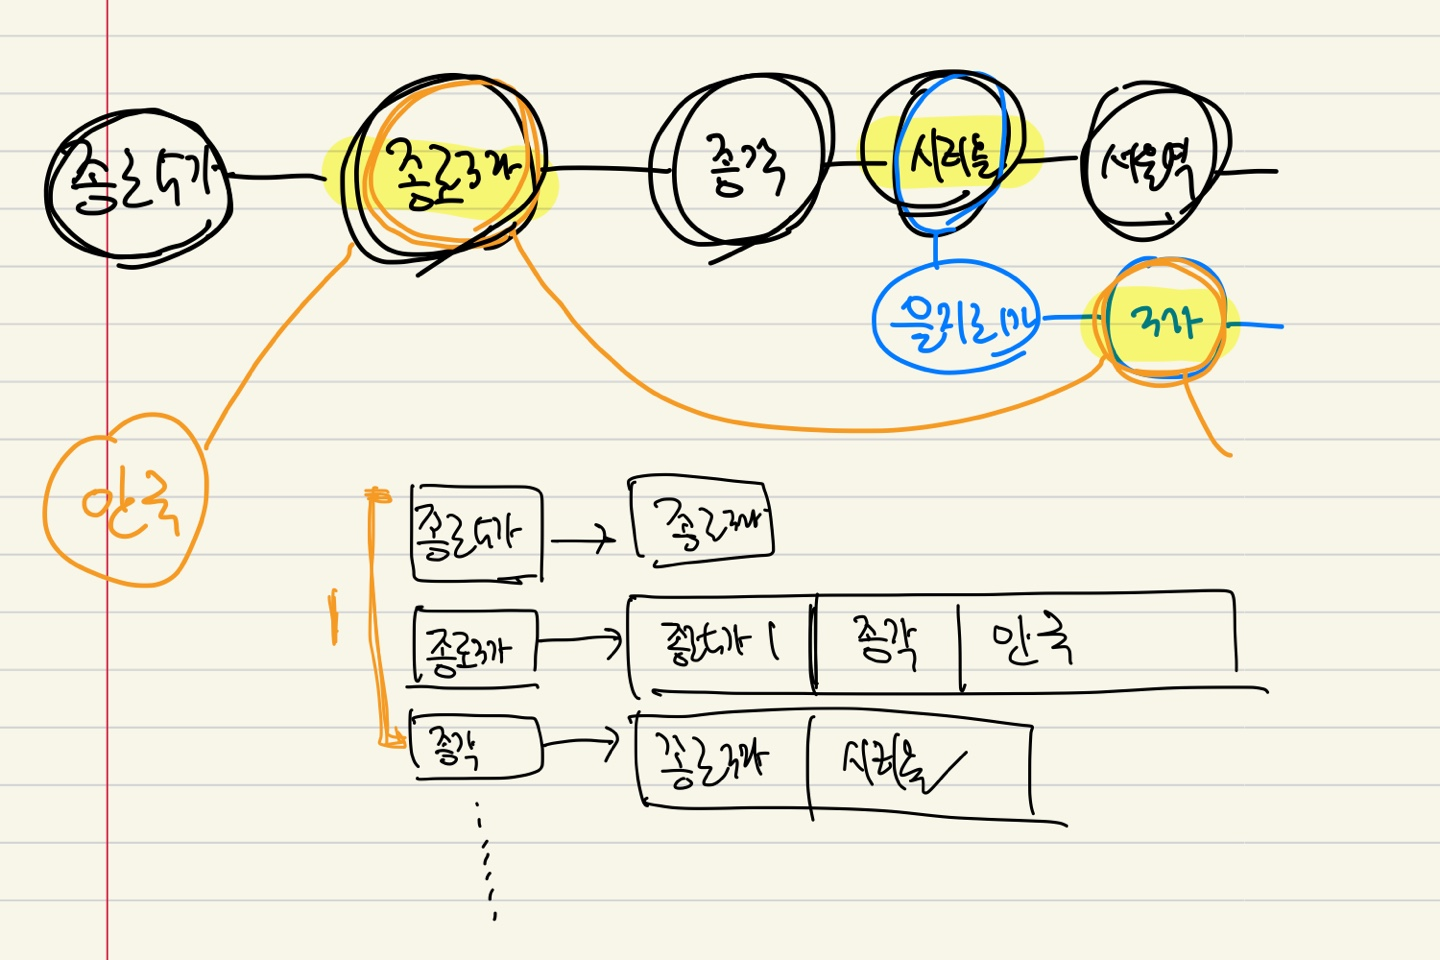
\includegraphics[width=0.4\textwidth]{expressWithList}
\caption{initial}
\label{fig:fig4}
\end{center}
\end{figure}


교재의 인접리스트와 그려둔 걸 토대로 비교해보니, 헤드노드에는 인덱스로 접근해야한다는 사실을 알 수 있었다. 실제로 값을 갖고 있는 것이 아니라 정점에 할당한 인덱스를 기준으로 같은 헤드노드 중 같은 인덱스가 그 정점이라고 생각해야하는 것이다. 따라서 Vertex클래스에 인덱스를 추가해줄 필요가 있었다. 

그 다음에 한 것은 리스트를 어떻게 구현할 것인가 였는데, 리스트를 사용하는 이유가 이중배열로 표현하면 불필요한 공간이 이용되기 때문이지 리스트에서 삽입하고, 삭제하는 등의 기능을 이용하기 위함이 아니였기 때문에 배열과 비슷한 vector를 사용하면 되겠다라고 생각했다. 그래서 이중 vector를 사용하여 그래프를 구현하기로 하였다.

\begin{figure}[!h]
\begin{center}
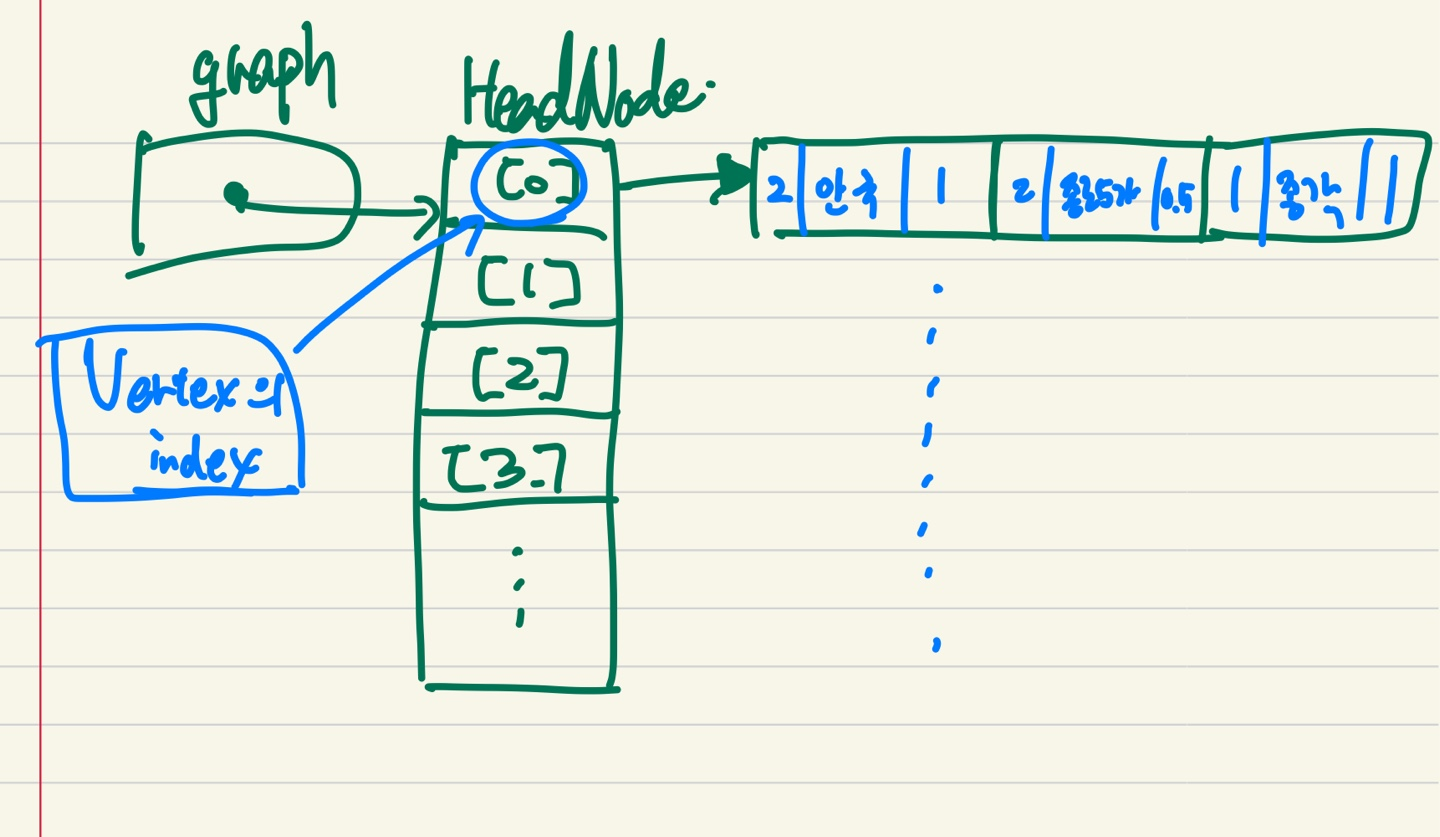
\includegraphics[width=0.4\textwidth]{implementationOfList}
\caption{implementation}
\label{fig:fig5}
\end{center}
\end{figure}


하나를 빼먹었던 것이 처음에 설계를 할 때, 최소비용트리와 최단거리를 착각하는 바람에 간선을 구현했었었고, 그 탓에 가중치를 담아둘 공간이 아예 없었다. Vertex 클래스에 dist에 가중치를 저장하게끔 했다. 

이후에 구현하면서 설계와는 다르게 추가되고 제거되었고, 최종적으로 다음과 같이 되었다.

\begin{Verbatim}
class Vertex
{
private:
    int line;       //호선
    string station; //역이름
    int dist;   //가중치
    int index;
public:
    Vertex()
    {
        line = 0;
        station = "\0";
    };
    Vertex(int line, string station);
    int getLine() { return line; };
    string getStation() { return station; };
    bool operator==(Vertex ver2)        //비교연산자
    {
        if (this->line == ver2.line && this->station == ver2.station) //호선도, 역도 같으면
            return true;
        else
            return false;
    };
    void setDist(Vertex &v);
    void setIndex(int index){ this->index = index; };
    int getIndex(){ return this->index; };
    int getDist(){ return this->dist; };
};

class Graph
{
private:
    int numOfVertex;	
    vector<int> dist; //거리 배열
    //vector<bool> check;
    vector<vector<Vertex> > HeadNodes;
    vector<Vertex> vertex; //모든 정점의 집합
    vector<int> route;
public:
    //int choose(const int n);
    Graph(int numLine, istream &f);
    void findShortestWay(int fromIndex, int toIndex);             //A부터 B로가는 최단거리
    void findFairPoint(int terminal1, int terminal2); //A와 B 중간의 지점
    int findIndex(Vertex station);         //graph에서 사용할 인덱스 찾아주는 함수
    bool isVertexExist(Vertex station);    //역이 이미 입력된적이 있는지 찾아주는 함수
    void printShortestWay(int fromIndex, int toIndex);
};
\end{Verbatim}

\section{결과값}
\textbf{test case 1}
\begin{Verbatim}
Anguk           //입력받은 시작점
Jongno_3(sam)-ga
Jonggak
City_Hall
Chungjeongno		//입력받은 종착점
5:00			//시점에서 종점까지의 시간
Jonggak			//공평한 지점
2:30				
2:30
\end{Verbatim}
\textbf{test case 2}
\begin{Verbatim}
Incheon		//입력받은 시작점
Dongincheon
Dowon
Jemulpo
Dohwa
Juan
Ganseok
Dongam
Baegun
Bupyeong
Bugae
Songnae
Jung-dong
Bucheon
Sosa
Yeokgok
Onsu
Oryu-dong
Gaebong
Guil
Guro
Sindorim
Yeongdeungpo
Singil
Daebang
Noryangjin
Nodeul
Heukseok
Dongjak
Gubanpo
Sinbanpo
Express_Bus_Terminal
Seoul_Nat'l_Univ._of_Education
Nambu_Bus_Terminal
Yangjae
Maebong
Dogok
Daechi
Hangnyeoul
Daecheong
Irwon
Suseo
Garak_Market
Nat'l_Police_Hospital
Ogeum		//입력받은 종착점
45:00		//걸린시간
Daerim		//공평한 지점
22:30
22:30
\end{Verbatim}
\section{기타}
\begin{itemize}
\item 범위기반 for문을 사용해서 구현한 함수가 있었는데, 한동안 vscode에서 여러개의 파일을 주는 방법을 몰라서 학교 리눅스 서버에서 컴파일을 하려고 했는데, 범위기반 for문이 C++98에서 지원이 안되는 것을 알았다.
\item vector와 stack, queue 모두 자료구조를 하기 전까지는 잘 안써봤기 때문에 모든 것이 생소했다. 각각을 다 알고 이해하는 것은 불가능하다고 생각했기때문에 필요한 만큼만 찾고 이용했다. stack은 다행히도 pop,push정도의 간단한 작업이면 충분했지만, vector는 아예 처음 사용해보는데다가, vector는 알아서 공간을 할당해준다! 라고 알고있어서 인덱스로 마음 편하게 접근했다가 segmentation fault도 수도 없이 겪었었다. 왜 안되나하고 한참을 씨름했었는데 할당된 공간과 vector의 size는 별개라는 것을 알게되었다. 또 처음에는 이중벡터를 구현하기위해서 vector$<$T$>$* 로 해둔 다음 동적할당을 햇었는데, 계속 안되길래 중단점을 설정하고 보니 할당이 안되는 것이였다. 그래서 결국 vector$<$vetor$<$T$>$$>$로 구현했었다. 그래도 나머지는 배열과 크게 다르지 않았기 때문에 다행이였다. 우선순위큐도 처음에 많이 헤맸었다. 다양한 기능을 쓴 것은 아니였지만, pair의 우선순위 큐는 어떻게 할 것이며, 오름차순으로 정리할지, 내림차순으로 정리할지, pair의 값은 두개인데 무슨 기준으로 정렬을 하는지 부터 모르는게 많았었다. 
\item 반복자의 사용이 어색하고 어려웠었다. 
\item 시간을 표현하는 것이 문제였는데, 예전에 c언어를 공부할 때였나, 비슷한 상황을 겪었던 것 같아서 시간을 최대한 보면서 기억을 되살리려고 했었다. 기억이 나지는 않았지만, 시간이 1분과 30초 두 종류 뿐인 것을 알았고, 2배인 것을 알 수 있었다. 그렇다면 환승역에는 1을 다른 경우에는 2를 가중치로 추가해서 그 합을 2로 나눠 몫과 나머지로 하면 되겠다 싶었다. 표현을 하고 돌려보니 생긴 문제는 30초인 경우에는 문제가 없었지만 0초인 경우 :0으로 나오는 것이였다. c언어에서야 형식지정자도 배우고 여러번 해봤지만, cout같은 경우에는 어떻게 저걸 :00으로 해야할지 전혀 몰랐다. 검색을 하고 setfill같은 나는 안되는 이상한 것들도 보았고 이것저것 시도해보면서 되는 방법을 찾았다. 
\item 알고리즘의 이해와 구현 역시도 어려웠다. 교재와 인터넷에 설명, 의사코드, 코드들이 즐비하니까 알고리즘의 구현을 어렵잖게 할 수 있었지만, 설명만 주어져있을 때 구현을 하는 것은 상당히 막막할 것 같았다. 
\end{itemize}
\end{document}